%!TEX root = /Users/markelikalderon/Documents/Git/formwithoutmatter/aristotle.tex
\chapter{Empedocles} % (fold)
\label{cha:empedocles}

\section{Dialectic} % (fold)
\label{sec:dialectic}

The present essay is about Aristotle's dialectical engagement with Empedocles concerning the nature of color perception. It is only by paying careful attention to such engagement can we arrive at a proper understanding of Aristotle's notorious definition of perception as the assimilation of the sensible form without the matter of the perceived object. I shall argue that Aristotle's definition of perception is a resolution of a puzzle or \emph{aporia} about the nature of perception that animated Empedocles' theory of vision. The puzzle concerns the sensory presentation of remote sensible objects, as when we see the colors of remote external particulars such as the brilliant white of the distant sun. This chapter details the original form of Empedoclean puzzlement and shows how Empedocles' theory of vision is an attempt to resolve such puzzlement, though an attempt that, as we shall see in chapter~\ref{cha:perception_at_a_distance}, Aristotle rejects as unworkable. But before we discuss the puzzle which animates Empedocles' theory of color vision, it will be useful to briefly describe Aristotle's dialectical engagement with the \emph{endoxa} more generally.

Dialectical argument is a mode of reasoning that uses the \emph{endoxa} as premises. The \emph{endoxa} are reputable opinions. The reputable opinions:
\begin{quote}
	\ldots\ are accepted by everyone or by the majority or by the wise---i.e. by all, or by the majority, or by the most notable and reputable of them. (Aristotle, \emph{Topica} \textsc{i} 1 101\( ^{a} \)35--37; Pickard-Cambridge in \citealt[2-3]{Barnes:1984uq})
\end{quote}
The opinions of the many and the wise are the source of both truth and error. Dialectical argument contrasts, in this way, with geometrical demonstration. Geometrical demonstration begins, not with the opinions of predecessors which may be a source of truth or error, but with premises that are primitive truths.

That the relevant opinions are widespread or are offered by the wise at least makes it likely that some element of truth is to be found among them. This is important insofar as dialectical argument is an alethic activity:
\begin{quote}
	For the study of the philosophical sciences it is useful, because the ability to puzzle on both sides of a subject will make us detect more easily the truth and error about the several points that arise. (Aristotle, \emph{Topica} \textsc{i} 2 101\( ^{a} \)35--37; Pickard-Cambridge in \citealt[3--4]{Barnes:1984uq})
\end{quote}
Dialectical argument thus serves a dual purpose. On the one hand, it makes it easier to discern what truth there is in the respected opinions of the predecessors. On the other hand, it makes it easier to eschew the errors of these same predecessors. Within the context of philosophical inquiry, then, dialectical argument is a means of determining the truth and avoiding error. If that is right, then this leaves open the possibility that at least some of what Empedocles has to say is true, at least on some understanding of what was said---though not necessarily Empedocles'. Thus, for example, in chapter~\ref{cha:the_eye}, we shall see how Aristotle accepts Empedocles' analogy between the eye in seeing and a lantern \textsc{dk} 31\textsc{b}84 but only on a novel understanding of that analogy. And in chapter~\ref{cha:form_without_matter}, we shall see that while Aristotle accepts the Empedoclean claim that perception is a mode of assimilation, he has a very different understanding of what assimilation involves in perceptual experience.

Dialectical argument proceeds by first collecting and organizing the respected opinions of one's predecessors and then by developing certain puzzles or \emph{aporiai} concerning the opinions that have been collected. These difficulties or puzzles either arise directly from the opinions of the many or the wise---when they conflict, say---or is the result of the development of these opinion with material external to the \emph{endoxa}. Determining, as best one can, what the appropriate resolution of such difficulties would be, is a means of avoiding the errors in the \emph{endoxa} while importantly preserving what insights there are as one advances one's judgment.

In the \emph{Metaphysica}, Aristotle describes the epistemic significance of dialectical argument for philosophical inquiry:
\begin{quote}
	For those who wish to get clear of difficulties it is advantageous to state the difficulties well; for the subsequent free play of thought implies the solution of the previous difficulties, and it is not possible to untie a knot which one does not know. But the difficulty of our thinking points to a knot in the object; for in so far as our thought is in difficulties, it is in like case with those who are tied up; for in either case it is impossible to go forward. Therefore one should have surveyed all the difficulties beforehand, both for the reasons we have stated and because people who inquire without first stating the difficulties are like those who do not know where they have to go; besides, a man does not otherwise know even whether he has found what he is looking for or not; for the end is not clear to such a man, while to him who has first discussed the difficulties it is clear. Further, he who has heard all the contending arguments, as if they were the parties to a case, must be in a better position for judging. (Aristotle, \emph{Metaphysica} \textsc{b} 1 995\( ^{a} \)27--995\( ^{b} \)4; Ross in \citealt[28]{Barnes:1984kx})
\end{quote}
Identifying and critically assessing such puzzles forces one to examine assumptions that may never have been questioned and yet may prove to be false. Moreover, unexamined false assumptions can hinder further investigation. In this way, dialectical argument is a means of avoiding error. Moreover, in identifying and assessing such puzzles one gains experience with the object of inquiry thus putting one in a better position to judge of its true nature. In this way, dialectical argument is a means for determining the truth. Thus in order be free from the distorting influence of false assumption as well as to be in a better position for judging the true nature of perception, Aristotle must first consider the difficulties that arise in the \emph{endoxa} concerning the nature of perception. 

In \emph{De Anima}, Book \textsc{i} is devoted to an elaborate and extended discussion of these difficulties as they arise with respect to the motion of the soul. In contrast to the characterization of the \emph{endoxa} given in \emph{Topica}, however, he restricts himself to the opinions of the wise as opposed to the many. Empedocles is prominent among the wise whose opinions are considered in Book \textsc{i}. However, it would be a mistake to see Aristotle's dialectical engagement with the \emph{endoxa} as confined to Book \textsc{i}. For example, \emph{De Anima} \textsc{ii} 5 begins by discussing an \emph{aporia} about alteration as it is understood by the \emph{endoxa}. Moreover, Aristotle's dialectical engagement with Empedocles is not itself confined to Book \textsc{i}, nor is his engagement with the reputable opinions of other predecessors, Plato being a prominent example. 

The puzzle with which we will be primarily concerned, a puzzle about the visual presentation of the colors of remote external particulars, is a puzzle to be found in the respected opinion of Empedocles. So it is a puzzle that arises strictly within the \emph{endoxa}, requiring no further development from without. Moreover, the \emph{endoxa}, here, seems restricted to the wise. However, this may, in the end, be misleading. Empedocles is attempting to reconcile certain aspects of the manifest image of nature with Parmenidean insights that may seem to conflict with it, and did so seem to Parmenides. Empedocles' theory of vision is part of this larger project. Empedoclean puzzlement arises from Empedocles' description of common phenomenological aspects of our experience of nature. Insofar as there are insights to be preserved in the respected opinion of Empedocles, the source of the puzzle described by Empedocles may lie with the way our sensory experience presents itself to be. But insofar as the source of the puzzlement lies, in part, with Empedocles description of sensory experience, then the puzzle arises from the way the wise articulates the phenomenology of the many. In any case, the focus is on the object of dialectical inquiry, in the present instance, the visual presentation of the colors of remote external particulars.

% section dialectic (end)

\section{The Answer in the Style of Gorgias} % (fold)
\label{sec:the_answer_in_the_style_of_gorgias}

In the \emph{Meno} Socrates attributes to Empedocles a conception of perception as a mode of assimilation of material effluences:
\begin{quotation}
    \textsc{meno}: And how do you define color?
    
    \ldots
    
    \textsc{socrates}: Would you like an answer in the style Gorgias, such as you most readily follow?
    
    \textsc{meno}: Of course I should.
    
    \textsc{socrates}: You and he believe in Empedocles' theory of effluences, do you not?
    
    \textsc{meno}: Wholeheartedly.
    
    \textsc{socrates}: And passages to which and through which the effluences make their way?
    
    \textsc{meno}: Yes.
    
    \textsc{socrates}: Some of the effluences fit into some of the passages whereas others are too great or too small.
    
    \textsc{meno}: That is right.
    
    \textsc{socrates}: Now you recognize the term `sight'?
    
    \textsc{meno}: Yes.
    
    \textsc{socrates}: From these notions, then, `grasp what I would tell,' as Pindar says. Color is an effluence from shapes commensurate with sight and perceptible to it. (Plato, \emph{Meno} 76\( ^{a-d} \); Guthrie in \citealt[359]{Hamilton:1989fk})
\end{quotation}

The main elements of the account are relatively clear. Objects emit material effluences. Effluences are fine bodies that are kind differentiated in terms of magnitude. There are passages in which and through which material effluences may flow. Whether a material effluence may enter a passage depends on its magnitude. The magnitudes of some kinds of material effluences are too great or too small for them to flow through a given passage. The magnitude of a material effluence must be commensurate with the magnitude of a passage in order for the effluence to fit the passage and so pass through it. Such passages exist in the membrane of the eye, thus allowing the eye to assimilate only a certain kind of material effluence, that is, the kind whose magnitude permits entry in ocular passages.

Thus we arrive at the answer in the style of Gorgias. That answer has three components. It specifies a kind of thing and two conditions that must be satisfied for a thing of that kind to be color. Color is (1) a kind of material effluence that is (2) commensurate with sight and (3) perceptible. First, color is a kind of material effluence, a chromatic effluence, say. Since material effluences are kind differentiated by magnitude, chromatic effluences have a distinctive magnitude. Second, chromatic effluences are commensurate with sight insofar as their distinctive magnitude permits entry in the passages of the membrane of the eye, the organ of sight. Notice, however, the assimilation of chromatic effluences by the organ of sight is not, by itself, the sensing of colors, otherwise the final condition would be redundant. The assimilation of chromatic effluence is at best a material precondition for their sensing. The thought seems to be this: In order for the chromatic effluences to be the object of sense, they first must be assimilated by the organ of sensation. It is only by assimilating chromatic effluences that they are presented to sight and are thereby seen. Socrates claims that the answer in the style of Gorgias may be generalized to the other sensory objects such as sound and smell (\emph{Meno} 76\( ^{d} \)), a claim echoed by Theophrastus' account of Empedocles (\emph{De Sensibus} \textsc{vii}). If that is right, then Empedocles, at least as presented by Socrates, is in the grip of a general conception of sensory awareness for which ingestion provides the model. Compare---in eating an olive, the matter of the olive is taken in and presented to the organ of taste and thereby tasted. On the ingestion model, to be perceptible is to be palpable to sense. 

The underlying thought is that in order for something to be the object of sense, it must be presented to the sense organ. On the ingestion model, it is a general feature that taste shares with paradigmatic cases of touch that is operative---the object of sensation must be in contact with the sense organ for it to be sensed. I say \emph{paradigmatic} cases of touch since it is arguable, at least, that one can feel something that one is not in direct contact with. (Thus one might feel the wooden frame of a Victorian rocking horse through the padding.) Theophrastus' commentary supports the suggestion that, according to Empedocles, an object must be in contact with the sense organ for it to be sensed (on the reliability of Theophrastus as a doxogapher see \citealt{Kahn:1994qf}). Following Aristotle's doxographic taxonomy (\emph{De Anima} \textsc{i} 2 404\( ^{b} \)12--15; cf \emph{Metaphysica} \textsc{b} 4 1000\( ^{b} \)5--8), Theophrastus counts Empedocles as a likeness theorist---as explaining perception in terms of the similarity of the elements that compose the object of sense and the sense organ. However, in \emph{De Sensibus} \textsc{xv}, Theophrastus concedes that Empedocles remains silent on the compositional similarity of the material effluence and the sense organ that assimilates it, emphasizing instead the role of contact in perception \citep{Kamtekar:2009fk,Sedley:1992uq}:
\begin{quote}
	For he attributes our recognition of things to two factors---namely, to likeness and to contact; and so he uses the expression ``to fit''. Accordingly if the smaller touched the larger ones, there would be perception. And likeness also, speaking generally, is out of the question, at least according to him, and commensurateness alone suffices. For he says that substances fail to perceive one another because their passages are not commensurate. But whether the effluence is like or unlike he leaves quite undetermined. (Theophrastus, \emph{De Sensibus} \textsc{xv}; \citealt[79]{Stratton:1917vn})
\end{quote}

To be perceptible is to be palpable to sense. If one began with that thought, a puzzle would naturally arise about vision, for vision seems to present the colors of distant objects. Color perception seems to involve the presentation of color qualities inhering in bounded particulars located at a distance from the perceiver. But how can one assimilate what remains inherent in a bounded particular remote from one? The puzzlement arise from the apparent tension between two claims:
\begin{enumerate}[(1)]
    \item The objects of color perception are qualities of external particulars located at a distance from the perceiver.
    \item \emph{The Empedoclean principle}: To be perceptible is to be palpable to sense---in order for something to be the object of perception it must be in contact with the relevant sense organ.
\end{enumerate}
I conjecture that, whatever independent reasons Empedocles may have had for believing in material effluences, it is precisely this puzzlement that effluences are meant to address in his theory of vision. The basic idea is simple enough, at least in broad outline. Distant objects may be sensed by sensing the material effluences they emit. If the color of an object is the material effluence that it emits, then the color of a remote object can be assimilated and so be palpable to sight. In this way, we can see the color of a bounded particular remote from us  consistent with the constraints imposed by the ingestion model. 

One may wonder whether the theory of effluences is wholly adequate to this task, at least without supplementation. Can we really see remote colored particulars on Empedocles's theory of vision, or are these occluded from view by the chromatic effluences they emit? Thus a Berkelean worry naturally arises about the immediate objects of sensation, the assimilated effluences, screening off the external objects that emit them. Moreover, it is not just colored objects that appear at a distance, but the colors themselves seem somehow confined to the remote bounded region in which they inhere. This aspect of color phenomenology is unexplained and perhaps inexplicable if sensed color is an effluence palpable to the perceptive part of the soul located within. Finally, there is a worry that in identifying colors with kinds of material effluences, Empedocles conflates ontological categories. Effluences are material bodies, but colors are not bodies, not even very fine bodies. Colors are, instead, qualities that could not exist apart from the bodies in which they inhere, at least according to the \emph{Categoriae}. (Not only does Aristotle have the resources to press this objection, but, as we shall see, when the same issue arises with respect to light, he adopts a parallel position, that light is not a body but a state, chapter~\ref{sec:transparency_in_de_anima}.) Fortunately, it is the puzzle that arises from Empedocles' conception of sensory presentation, and not his resolution of it, that is our focus here. 

% section the_answer_in_the_style_of_gorgias (end)

\section{Empedocles' Theory of Vision} % (fold)
\label{sec:empedocles_theory_of_vision}

Empedocles' own theory of color vision is more elaborate than the answer in the style of Gorgias. Despite being more elaborate, the ingestion model remains at the core of that theory. 

One element missing from the account that Socrates offers to Meno is the eye's emission of fiery effluences. That effluences may flow out of passages as well as in is consistent with, if not indeed suggested by, Socrates' general description of passages ``to which and through which'' effluences may flow. This is worth considering, since it can seem to offer an explanation that conflicts with the explanation of color vision in terms of the assimilation of material effluences. And while Aristotle notes the apparent tension, Theophrastus provides the basis for understanding the role the emission of fiery effluences plays in the assimilation of chromatic effluences.

Aristotle (\emph{De Sensu} \textsc{ii} 437\( ^{b} \)27--438\( ^{a} \)3) cites the following passage from Empedocles:
\begin{verse}
	As when someone planning a journey prepared a lamp,\\
	the gleam of blazing fire through the wintry night,\\
	and fastened linen screens against all kinds of breezes,\\
	which scatter the wind of the blowing breezes\\
	But the light leapt outwards, as much of it as was finer,\\
	and shone with its tireless beams across the threshold;\\
	in this way [Aphrodite] gave birth to the rounded pupil,\\
	primeval fire crowded in the membranes and in the fine linens.\\
	And they covered over the depths of the circumfluent water\\
	and sent forth fire, as much of it as was finer.\\
	(Empedocles, \textsc{dk} 31\textsc{b}84; \citealt[103 259]{Inwood:2001ve})
\end{verse}
On this basis, Aristotle maintains that, like Plato in the \emph{Timaeus}, Empedocles explains vision in terms of the emission of fire. But then he remarks ``Sometimes he accounts for vision thus, but at other times he explains it by emanations from the visible objects'' (\emph{De Sensu} \textsc{ii} 438\( ^{a} \)3--4; Beare in \citealt[5]{Barnes:1984uq}). So, at the very least, Aristotle thinks that Empedocles is potentially offering distinct explanations of color vision---one in terms of the eye's emission of a fiery effluence and the other in terms of the eye's assimilation of chromatic effluences. But if Empedocles explains vision by the assimilation of chromatic effluence, why does he also need the emission of a fiery effluence? Is Empedocles really offering conflicting explanations of vision? 

In the passage cited by Aristotle, Empedocles describes the anatomy of the eye by analogy with an artifact, a screened lamp, constructed from linen or shaved horn, say (on interpreting the composition of the screen see \citealt[240--241]{Wright:1981zr}). Interpreting the screen as composed of linen has the advantage of more closely echoing the fine membrane that Aphrodite weaves. Just as there is fire in the interior of a screened lamp, there is a primeval fire in the interior of the eye, or perhaps the pupil. And just as the screen of linen or shaved horn surrounds the fire in the lamp's interior, there is a membrane that surrounds the fire in the eye's interior. Moreover, the membrane plays a similar role to the screen. Just as the screen protects the interior fire from the wind which would extinguish it, the primeval fire is protected from the depth of the surrounding water by the membrane of the eye. Finally, just as light passes through the screen, the primeval fire can pass through passages in the membrane of the eye. 

What is the surrounding water? Some commentators maintain that the membrane separates interior fire from interior water. Other commentators maintain that the membrane separates interior fire from exterior water. On the former interpretation, the membrane divides the eye's interior, and the surrounding water is the vitreous humor (\citealt[16]{Beare:1906uq}; \citealt[241--242]{Wright:1981zr}). On the latter interpretation, the membrane surrounds the eye, and the surrounding water is the lachrymal fluid on the surface of the eye \citep{Sedley:1992uq}. The former interpretation is supported by Theophrastus' (\emph{De Sensibus} \textsc{xv}) attribution of interior water and interior fire to the eye. On the other hand, if we take seriously one particular aspect of the analogy, that the surrounding water is like the wind in being external, then it is hard to understand the surrounding water as anything other than lachrymal fluid. So presented, these interpretations can seem like stark alternatives. However, a hybrid interpretation is possible. On the hybrid interpretation, interior fire and water are separated from one another and from exterior water by means of the eye's membrane (\citealt[326]{Lloyd:1966ly}; \citealt[26 n39]{Ierodiakonou:2005fk}). On the hybrid interpretation, interior water is the vitreous humor and exterior water is the lachrymal fluid. The evidence for the alternative interpretations equally support the hybrid interpretation, and I adopt it here as a working hypothesis.

Why must fiery effluences be emitted if the eye is to assimilate chromatic effluences? Theophrastus offers the basis of an explanation:
\begin{quote}
	The passages <of the eye> are arranged alternately of fire and of water: by the passages of fire we perceive white objects; by those of water, things black; for in each of these case <the objects> fit into the given <passage>. Colors are brought to our sight by an effluence. (Theophrastus, \emph{De Sensibus} \textsc{vii}; \citealt[71--73]{Stratton:1917vn})
\end{quote}
How are we to understand the passages of the eye being arranged alternately of fire and water? Here is a simple model that coheres with the text (perhaps not the only one): Picture the passages in the membrane of the eye as being arranged in a regular array (see Figure~\ref{fig:1}). There are two kinds of passages, fire passages and water passages. Each kind of passage is adjacent to the alternate kind of passage. So fire passages are always adjacent to water passages and water passages are always adjacent to fire passages. Fire passages are passages in the membrane of the eye lined with fire emitted from the interior. This has the effect of narrowing the passage, thus allowing only smaller effluences to pass, such as white effluences. Water passages are the passages in the eye that are not lined with fire. The magnitude of the surrounding water, the lachrymal fluid, is too great, say, to enter these passages. However, they count as water passages since any effluences entering them must pass through the surrounding water. Water passages are wider than fire passages thus allowing the passage of effluences of greater magnitude, such as black effluences. In being commensurate with, respectively, the fire and water passages in the membrane of the eye, white and black effluences may be assimilated by the eye and so be palpable to sight. 

\begin{figure}[ht]
    \begin{center}
        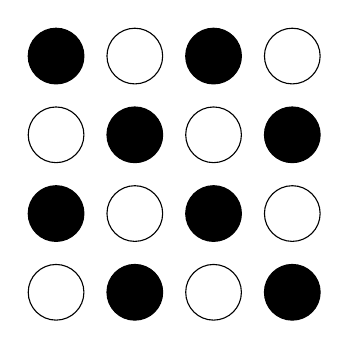
\begin{tikzpicture}
			[inner sep=2.5mm,
			fire/.style={circle,draw},
			water/.style={circle,draw,fill=black}]
			\path node at (0,0) [fire]  {}
				  node at (0,1) [water] {}
				  node at (0,2) [fire]  {}
				  node at (0,3) [water] {}
				  node at (1,0) [water] {}
				  node at (1,1) [fire]  {}
				  node at (1,2) [water] {}
				  node at (1,3) [fire]  {}
				  node at (2,0) [fire]  {}
				  node at (2,1) [water] {}
				  node at (2,2) [fire]  {}
				  node at (2,3) [water] {}
				  node at (3,0) [water] {}
				  node at (3,1) [fire]  {}
				  node at (3,2) [water] {}
				  node at (3,3) [fire]  {};
		\end{tikzpicture}
    \end{center}
    \caption{Array of fire and water passages in the membrane of the eye. Fire passages are white, water passages are black.}
    \label{fig:1}
\end{figure}

Against the present model, one might object that the fire and water passages in the membrane of the eye are so called because of the elemental composition of the effluences that are commensurate with them. Thus fire passages only admit fiery effluences, and water passages only admit watery effluences. This is a plausible explanation of Empedoclean nomenclature and coheres well with Theophrastus claim that the eye, as conceived by Empedocles, consists of ``fire and its opposite''. However, at least by itself, the suggestion fails to reconcile the answer in the style of Gorgias with the eye's emission of fiery effluences. Fortunately, it is less a genuine alternative to the present model than a plausible supplement. Suppose, then, that fire is the elemental composition of white effluences and that water is the elemental composition of black effluences. The smaller fiery effluences are commensurate only with the fire passages, the passages lined with fire, and the larger watery effluences are commensurate only with the water passages, the passages not so lined. The fire passages lead to the primeval fire within, itself confined and bound by a fine membrane. Just as fire passages lead to fire in the eye's interior, water passages lead to water in the eyes' interior. And each are bound and separated from one another by the fine membrane Aphrodite wove.

If black effluences are composed of water and their magnitude is commensurate with the water passages in the membrane of the eye, how is it that the surrounding water, the lachrymal fluid, does not leak through? How is it that watery effluence and not the surrounding water is commensurate with water passages? While effluences may be kind differentiated in terms of magnitude, perhaps these kinds are not aligned with elemental divisions. Fine bodies composed of water may differ in magnitude, and so constitute different kinds of effluence. The surrounding water, due to its greater magnitude, say, is not commensurate with the water passages in the membrane of the eye. That is how Aphrodite's Love constrains them. Only a certain kind of watery effluence is commensurate with ocular passages, the kind of watery effluence emitted by distal objects and that constitute the color of the objects that emit them. 

Moderns will react to this model with a mixture of familiarity and strangeness. The idea of an array of different kinds of receptors is familiar from vision science. The strangeness, for us, is that Empedocles places this array on the surface of the eye instead of the retinal interior \citep[for a comparison of Empedocles' theory with modern theories of vision see][]{Siegel:1959fk}. This strangeness ought not to blind us to the way in which Empedocles' view is, nevertheless, a respectable piece of natural philosophy. Specifically, Empedocles view coheres well with the dominant medical opinion of his time. Arguably, it was designed to so cohere. The presence of lachrymal fluid is both necessary for sight and necessary for the reflective appearance of the eye. This encouraged the opinion that the reflective appearance of the eye explained the eye's capacity for sight, and hence that the surface of the eye is the locus of sight. (Consider the view that Aristotle attributes to Democritus, \emph{De Sensu} \textsc{ii} 438\( ^{a} \)5ff.) Notice how this can seem inconsistent with the ingestion model. On the ingestion model, the interior of the eye is the locus of sight. Empedocles' own more elaborate theory can be motivated, in part, by the reconciliation it offers. Empedocles' reconciles the ingestion model to the dominant medical opinion of his day by conceiving of the receptors on the surface of the eye as water-bound passages to its interior.

Even taking the model on its own terms, questions remain. The perception of black and white is relatively straightforward. White effluences emitted from distal objects are assimilated through fire passages, black effluences emitted from distal objects are assimilated through water passages, and so each is made palpable to the organ of sight. But what about the perception of the other hues? How, on this model, is the perception of red explained? Theophrastus complains that Empedocles owes us an explanation but fails to provide one:
\begin{quote}
	Now since, for him, the eye is composed of fire and of its opposite, it might well recognize white and black by means of what is like them; but how could it become conscious of gray and the other compound colours? For he assigns <their perception> neither to the minute passages of fire nor to those of water nor to others composed of both these elements together. Yet we see the compound colours no whit less than we do the simple. (Theophrastus, \emph{De Sensibus} \textsc{xvii}; \citealt[81]{Stratton:1917vn})
\end{quote}
Perhaps the perception of red can be explained in terms of the ratio of black and white assimilated \citep{Ierodiakonou:2005fk}. So understood, Empedocles anticpates, in this way, Aristotle's account of the generation of the hues, \emph{De Sensu} \textsc{iii} 439\( ^{b} \)ff. This Aristotelian hypothesis at least has the virtue of explaining the perception of chromatic hues only in terms of elements already present in the model. That the elements of the model should prove sufficient for the perception of color quite generally is suggested by the concluding line of Theophrastus' description of that model: ``Colors are brought to our sight by an effluence''. In the passage cited by Aristotle (\emph{De Sensu} \textsc{ii} 437\( ^{b} \)27--438\( ^{a} \)3; Empedocles \textsc{dk} 31\textsc{b}84), the Love that binds the primeval fire in the eye's membrane is Aphrodite's Love and is the principle of harmony. If the perception of red is due to the ratio of black and white among the assimilated effluences, then the perception of red is due, in part to the principle of harmony. Could Aphrodite's Love take so marvelous a form? (We shall return to this question in chapters~\ref{cha:light_and_dark} and \ref{cha:the_generation_of_the_hues}.)

Empedocles own theory of color vision is more elaborate than the answer in the style of Gorgias. Despite being more elaborate, the ingestion model remains at the core of that theory. Theophrastus' insight is that the emission of fiery effluences is not an alternative account of color vision as Aristotle supposed, but a necessary precondition for the assimilation of chromatic effluences. So even on Empedocles' more elaborate theory of color vision, a conception of sensory awareness as a mode of assimilation remains at its core. Key features of that theory are driven by the central principle of the ingestion model, the Empedoclean principle, to be perceptible is to be palpable to sense.

% section empedocles_theory_of_vision (end)

\section{Empedoclean Puzzlement} % (fold)
\label{sec:empedoclean_puzzlement}

I believe that Empedocles' puzzlement about the sensory presentation of the remote objects of sight is a natural one. The puzzlement survives abandoning what surely is the immediate culprit in the ingestion model, the principle that to be perceptible is to be palpable to sense. 

Indeed, Empedoclean puzzlement persists at least well into the twentieth century. Thus Bergson remarks:
\begin{quote}
	A man born blind, who had lived among others born blind, could not be made to believe in the possibility of perceiving a distant object without first perceiving all the objects in between. Yet vision performs this miracle. In a certain sense the blind man is right, since vision, having its origin in the stimulation of the retina, by the vibrations of the light, is nothing else, in fact, but a retinal touch. \citep[168]{Bergson:1907sh}
\end{quote}
But how can retinal touch perceive distant objects without first perceiving the objects between? Indeed, how can retinal touch perceive distant objects at all? Bergson never explains how this miracle is brought off. Less than half a century later, Broad reports a similar puzzlement:
\begin{quote}
    It is a natural, if paradoxical, way of speaking to say that seeing seems to `bring us into \emph{contact} with \emph{remote} objects' and to reveal their shapes and colors. \citep[33]{Broad:1952kx}
\end{quote}
This natural if paradoxical way of speaking is ubiquitous among contemporary philosophers of perception, but the miraculous character of the phenomenon goes largely unremarked. A recent notable exception is \citet{Valberg:1992aa}. Valberg addresses a puzzle that arises about the sensory presentation of distal objects if sensory experience is located where the perceiver is:
\begin{quote}
	How could the man `out there', at a distance from my head, be present in my experience, if my experience is something which is occurring `back up here', inside my head? \citep[141]{Valberg:1992aa}
\end{quote}

In its most general form, the puzzlement about how one may be in perceptual contact with remote objects is but one aspect of the problem discussed by contemporary philosophers under the rubric of presence in absence. The puzzlement consists in an inability to understand how to coherently combine the distal character of the objects of sight with a conception of sensory awareness as a mode of assimilation. It would be premature to dismiss that conception, even in its original Empedoclean form, as primitive physiology of vision. Indeed, Aristotle retains the conception of perception as a mode of assimilation even as he transforms it in rejecting Empedocles' theory of effluences. Aristotle retains that conception presumably because he felt that there was an insight that should be preserved in Empedocles' opinion. 

Aristotle is not alone in thinking that there is an insight to be preserved in conceiving of sensory awareness as a mode of assimilation. Thus \citet{Broad:1952kx} speaks of the presentation of the objects of visual awareness as a mode of prehension.  ``Prehension'' belongs to a primordial family of broadly tactile metaphors for sensory awareness that includes ``grasping'', and ``apprehending''. What unites these metaphors is that they are all a mode of assimilation, and ``ingestion'' is a natural variant \citep[see][7]{Johnston:2006uq,Price:1932fk}. For what it is worth, assimilation as a metaphor for perception is inscribed in the history of the English language. The word ``perception'' derives from the Latin \emph{perceptio} meaning to take in, or assimilate \citep[102]{Burnyeat:1979mv}---evidence, at least, for the persistence of an inclination. It is natural, then, to think of seeing as taking in the external scene before one. But then the question arises: How can one take in what remains external? And if one can, what could taking in mean, here, such that one could? Empedoclean puzzlement, in its most general form, consists in the persistence of this latter question.

It is worth wondering about the prevalence of tactile metaphors for visual awareness. There is an Aristotelian explanation, I think. The explanation is Aristotelian, not in the sense that Aristotle gives the explanation or even entertains it. Rather, it is Aristotelian in that it draws on resources available in Aristotle's thought. 

According to Aristotle, taste and touch are primitive forms of sensation common to all animals (though animals can and do differ in their possession of other sensory capacities). Whereas the objects of the distal senses are for the animal's well-being, the objects of touch concern the animal's very existence (\emph{De Anima} \textsc{iii} 13 433\( ^{b} \)31--434\( ^{a} \)10). What we touch may put us in mortal danger or provide us with vital sustenance. Touch is primitively compelling because of its existential character.

Suppose then, at least in human beings, the primitive character of touch is manifest in our emotional responses to things. Often when we see something we are drawn to touch it, even though there is no doubt about its presence or solidity. It is as if a thing's presence is most keenly felt when grasped. Thus we must endeavor to teach children to keep their hands to themselves, and even in maturity, polite notices are required to remind adults to not touch the display cabinet. 

Grasping is sufficiently phenomenologically compelling that it becomes, in the cosmology of the Giants, a touchstone for reality. Thus in the \emph{Sophist} the Eleatic Visitor reports: 
\begin{quote}
    One party is trying to drag everything down to earth out of heaven and the unseen, literally grasping rocks and trees in their hands, for they lay hold upon every stock and stone and strenuously affirm that real existence belongs only to that which can be handled and offers resistance to the touch. (Plato, \emph{Sophist} 246\( ^{a} \); Cornford in \citealt[990]{Hamilton:1989fk})
\end{quote}
If real existence belongs only to that which can be handled and offers resistance to touch, then only the palpable is real. Sensory perception is a mode of awareness. Awareness must be an awareness of what is real if it is to be awareness at all. It follows that the objects of perception must themselves be palpable. It is a further claim, however, that not only are the objects of perception palpable, but they are palpable, as well, to the organ of sense, in the way that Empedocles requires. Sensory perception presents itself as a mode of awareness of particulars arrayed in the natural environment. And the Empedoclean thought would be that perception could only be as it presents itself to be if its objects were palpable to the organ of sense. But even if real existence belongs only to that which can be handled and offers resistance to touch, it does not follow that the perceptible must be palpable to sense. Grasping may manifestly be a mode of sensing, but it does not follow that it is the only mode, or that all modes of sensory presentation must be understood on its model. The Giants' metaphysical principle, only the palpable is real, may not entail the Empedoclean principle, to be perceptible is to be palpable to sense, nevertheless the appeal of these distinct principles flow from a common source, the vivid and primitively compelling phenomenology of an external particular's resistance to touch.

If the presence of things is most keenly felt when grasped, if in the resistance to touch their presence is manifest in a primitively compelling manner, then it would be no surprise that we reach for tactile metaphors in characterizing sensory presentation, even as it figures in nontactile modes of sensory awareness such as vision. If the Aristotelian explanation is correct, then the tactile metaphors are emphasizing the \emph{presentation} of the objects of sensory awareness. It is because objects grasped are presented to us in a primitively compelling manner, that grasping can serve as a paradigm of sensory presentation. On the Aristotelian explanation, the palpable is real---touch is a genuine mode of sensory awareness. But neither the Giants' principle nor Empedocles' follows. The palpable may be real, but it is not the case that only the palpable is real. Aristotle accepts the Eleatic Visitor's observation that virtues and capacities are real if not palpable. Nor is it the case that only by being palpable to the organ of sense is an object perceptible. Indeed, Aristotle will argue that an object's contact with a sense organ precludes sensation.

If the Aristotelian explanation is correct, then Empedoclean puzzlement, in its original form,  is the result of overgeneralizing from a paradigm case. To be sure, vision involves the presentation of colors inhering in bounded particulars remote from the perceiver. But if the presentation of color in sensory consciousness is too closely modeled on a capacity to grasp or take in something material, then a puzzle arises that only the theory of effluences may resolve. If indeed it does. I have already mentioned three reservations: (1) the Berkelean worry about the immediate objects of perception, the assimilated effluences, screening off the distal objects that emit them; (2) that perceived color itself appears to inhere in the remote bounded region of the external particular; and (3) that colors belong to a different ontological category from material bodies. As we shall see in the next chapter, Aristotle has his own criticisms to make of Empedocles' theory of color vision. Far from being a necessary condition on perception, contact with the sense organ precludes perception. Placing a colored particular on the eye blinds the perceiver to the particular and its color (\emph{De Anima} \textsc{ii} 7 419\( ^{a} \)13--14). If Aristotle's criticism proves cogent, then Empedoclean puzzlement, in its original form, not only involves an overgeneralization from a paradigm case but a misconception of it as well. If to be palpable is to be imperceptible, then not even touch works by the object of sense being in contact with the sense organ. Grasping may be a paradigm case of sensory presentation, but not because it involves an object being in contact with a sense organ. Rather, it is a paradigm case because objects grasped are presented to us in a primitively compelling manner. But even if we resist the temptation to which Empedocles apparently succumbed, to overgeneralize, in this way, from a misconception of a paradigm case, there remains the question: What could the sensory presentation of qualities of remote external particulars be, if not simply their being palpable to sense?

% section empedoclean_puzzlement (end)

\section{Definition} % (fold)
\label{sec:definition}

In \emph{De Anima} \textsc{ii} 12 424\( ^{a} \)18--23, \textsc{ii} 5 418\( ^{a} \)3--6 Aristotle defines perception as a mode of assimilation of the sensible form without the matter of an external particular. This is an instance of Aristotle's dialectical refinement of the \emph{endoxa} \citep[on Aristotle's dialectic in \emph{De Anima} see][]{Witt:1995kx}. While denying that sight involves the assimilation of material effluences, Aristotle retains Empedocles' conception of sensory awareness as a mode of assimilation, it is just that we assimilate form without matter. Indeed, this pattern of dialectical refinement continues in the very next line where Aristotle uses Plato's metaphor of wax receiving an impression, not to characterize judgment as Plato does in the \emph{Theaetetus} 194\( ^{c} \)--195\( ^{a} \), but to characterize the assimilation of sensible form in perception. Given this pattern of dialectical refinement, we can be confident that Aristotle was engaging with Empedocles' thought in his definition of perception. And while it remains controversial how to understand the assimilation of sensible form, I believe progress can be made by interpreting Aristotle's definition of perception as addressing Empedocles' puzzlement about how remote objects can be present in sensory consciousness. Recall Empedoclean puzzlement begins with the natural thought that in seeing one takes in the external scene. The question then arises: How can we take in what remains external? And if one can, what could taking in mean such that one could? The proposal is to interpret Aristotle's definition of perception as an answer to this latter question---a remote object can be present in sensory consciousness by assimilating its sensible form while leaving its matter in place. Understanding how Aristotle's definition of perception so much as could be a resolution of Empedoclean puzzlement imposes a substantive constraint on interpreting that definition, for so interpreted, it is making an important claim about the metaphysics of sensory presentation.

Aristotle's definition of perception is a dialectical refinement of the \emph{endoxa} insofar as it seeks to preserve an Empedoclean insight while resolving a puzzle about how remote objects can be present to sensory consciousness. Empedocles' puzzlement about the nature of sensory presentation persists to this day, though now in the guise of discussions of presence in absence. Perhaps there are insights of Aristotle's own that ought to be preserved when confronting Empedoclean puzzlement as it arises in its modern guise. If there are, then a conception of sensory presentation that preserved Aristotle's insight into the proper resolution of Empedoclean puzzlement would itself be a dialectical refinement of the respected opinion of Aristotle. What these insights might be and whether any conception of sensory presentation answers this description remains to be determined.

% section definition (end)

% chapter empedocles (end)